\documentclass[tikz,border=6pt]{standalone}
\usepackage{tikz}
\usetikzlibrary{arrows.meta,calc}
\usepackage{dsfont}
\usepackage{newpxtext}
\usepackage{newpxmath}

\begin{document}
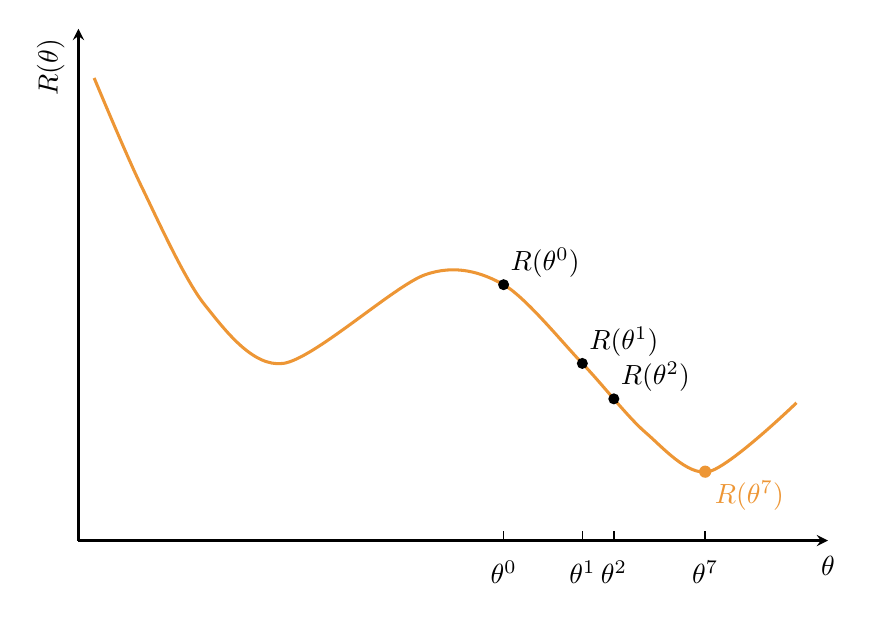
\begin{tikzpicture}[x=4cm,y=2.5cm]
  % colors
  \definecolor{curve}{RGB}{237,150,53} % warm orange

  % --- axes ---
  \draw[-stealth,line width=0.8pt] (-1.10,0) -- (1.28,0) node[below=2pt] {$\theta$};
  \draw[-stealth,line width=0.8pt] (-1.10,0) -- (-1.10,2.6) node[left=10pt,rotate=90] {$R(\theta)$};

  % --- loss curve (hand-sketched smooth path) ---
  \draw[line width=1.1pt,curve] 
    plot[smooth] coordinates{
      (-1.05,2.35)
      (-0.9,1.80)
      (-0.7,1.20)
      (-0.45,0.9)
      ( 0.00,1.35)
      ( 0.25,1.30)
      ( 0.50,0.9)
      ( 0.70,0.55)
      ( 0.90,0.35)
      ( 1.18,0.70)
    };

  % --- x positions for thetas (you can tweak these) ---
  \def\tzero{0.25}
  \def\tone {0.50}
  \def\ttwo {0.60}
  \def\tseven{0.89}

  % approximate R(theta) values on the drawn curve
  \def\Rzero{1.30}
  \def\Rone {0.90}
  \def\Rtwo {0.72}
  \def\Rsev {0.35}

  % --- tick marks and labels on x-axis ---
  \foreach \t/\lab in {\tzero/{$\theta^{0}$}, \tone/{$\theta^{1}$}, \ttwo/{$\theta^{2}$}, \tseven/{$\theta^{7}$}}{
    \draw[line width=0.6pt] (\t,0) -- ++(0,0.05);
    \node[below=4pt] at (\t,0) {\lab};
  }

  % --- points on the curve (black for first three, orange for final) ---
  \fill ( \tzero,\Rzero) circle (2pt);
  \fill (  \tone,\Rone ) circle (2pt);
  \fill (  \ttwo,\Rtwo ) circle (2pt);
  \fill[curve] (\tseven,\Rsev) circle (2.2pt);

  % --- text labels near the points ---
  \node[above right=-1pt] at ( \tzero,\Rzero) {$\small R(\theta^{0})$};
  \node[above right=-1pt] at (  \tone,\Rone ) {$\small R(\theta^{1})$};
  \node[above right=-1pt] at (  \ttwo,\Rtwo ) {$\small R(\theta^{2})$};
  \node[below right=0pt,curve] at (\tseven,\Rsev) {$\small R(\theta^{7})$};

\end{tikzpicture}
\end{document}
